\documentclass[5p]{elsarticle}

% --- packages ---
\usepackage{graphicx}
\usepackage{tikz}
\usetikzlibrary{positioning,arrows.meta}
\usepackage{booktabs}
\usepackage{url}

% \todo renders visibly so nothing is silently missing (no todonotes dependency).
\newcommand{\todo}[1]{\textbf{[TODO: #1]}}

% Single source of truth for every real number (macros only; no hand-typed figures).
% AUTO-GENERATED from repo data — DO NOT hand-edit numbers. Regenerate: node scripts (see papers/README).
% Every macro = a real measured value from the cited source file.

% ---- per-subject 5-fold CV mean accuracy (percent) ----
\newcommand{\AccOne}{86.7}% source: tests/fixtures/S001/cv_accuracy.json
\newcommand{\AccTwo}{86.7}% source: tests/fixtures/S002/cv_accuracy.json
\newcommand{\AccThree}{60.0}% source: tests/fixtures/S003/cv_accuracy.json
\newcommand{\AccFour}{68.9}% source: tests/fixtures/S004/cv_accuracy.json
\newcommand{\AccFive}{57.8}% source: tests/fixtures/S005/cv_accuracy.json
\newcommand{\AccSix}{33.3}% source: tests/fixtures/S006/cv_accuracy.json
\newcommand{\AccSeven}{93.3}% source: tests/fixtures/S007/cv_accuracy.json
\newcommand{\AccEight}{66.7}% source: tests/fixtures/S008/cv_accuracy.json
\newcommand{\AccNine}{35.6}% source: tests/fixtures/S009/cv_accuracy.json
\newcommand{\AccTen}{57.8}% source: tests/fixtures/S010/cv_accuracy.json
\newcommand{\AccMin}{33.3}% source: min over tests/fixtures/*/cv_accuracy.json
\newcommand{\AccMax}{93.3}% source: max over tests/fixtures/*/cv_accuracy.json

% ---- browser-vs-MNE agreement (machine precision) ----
\newcommand{\FilterR}{1.0}% source: tests/pipeline/multisubject.test.ts (filterR, 12 dp)
\newcommand{\CspFrobMin}{\ensuremath{6.6\times10^{-15}}}% source: multisubject test (CSP Frobenius)
\newcommand{\CspFrobMax}{\ensuremath{1.7\times10^{-14}}}% source: multisubject test (CSP Frobenius)
\newcommand{\LdaDiffMin}{\ensuremath{1.7\times10^{-13}}}% source: multisubject test (LDA weight diff)
\newcommand{\LdaDiffMax}{\ensuremath{2.4\times10^{-12}}}% source: multisubject test (LDA weight diff)

% ---- dataset / counts ----
\newcommand{\Nsubjects}{10}% source: tests/fixtures/subjects.json
\newcommand{\Nskipped}{0}% source: tests/fixtures/subjects.json
\newcommand{\Nepochs}{45}% source: tests/fixtures/*/params.json n_epochs
\newcommand{\Nchannels}{64}% source: params.json n_channels
\newcommand{\Fs}{160}% source: params.json fs_hz
\newcommand{\Ntimes}{321}% source: params.json epoch.n_times
\newcommand{\Ntests}{40}% source: npx vitest run (Test Files 13 / Tests 40)

% ---- method constants (match the code/oracle exactly) ----
\newcommand{\FirLo}{8}% source: params.json filter.cutoff_hz
\newcommand{\FirHi}{30}% source: params.json filter.cutoff_hz
\newcommand{\FirTaps}{165}% source: params.json filter.numtaps
\newcommand{\Tmin}{0.5}% source: params.json epoch.tmin_s
\newcommand{\Tmax}{2.5}% source: params.json epoch.tmax_s
\newcommand{\CspReg}{0.1}% source: params.json csp.reg
\newcommand{\CspComp}{4}% source: params.json csp.n_components
\newcommand{\LdaShrink}{0.1}% source: params.json lda.shrinkage
\newcommand{\Folds}{5}% source: params.json cv.n_splits
\newcommand{\Seed}{42}% source: params.json cv.random_state

% ---- oracle environment ----
\newcommand{\MneVer}{1.8.0}% source: subjects.json env
\newcommand{\SklearnVer}{1.5.2}% source: subjects.json env
\newcommand{\ScipyVer}{1.14.1}% source: subjects.json env
\newcommand{\NumpyVer}{2.0.2}% source: subjects.json env
\newcommand{\PyVer}{3.12.12}% source: subjects.json env

% ---- benchmark (real, reference run) ----
\newcommand{\WorkerOneX}{1696}% source: benchmarks/results.json conditionsWorker 1x
\newcommand{\WorkerOneXStd}{20}% source: benchmarks/results.json conditionsWorker 1x
\newcommand{\ProxyOneX}{1013}% source: benchmarks/results.json conditionsMain 1x
\newcommand{\ProxyFourX}{3954}% source: benchmarks/results.json conditionsMain 4x
\newcommand{\ProxySixX}{5992}% source: benchmarks/results.json conditionsMain 6x
\newcommand{\PeakHeap}{192.2}% source: benchmarks/results.json memory.peakMB
\newcommand{\BaseHeap}{9.0}% source: benchmarks/results.json memory.baseMB
\newcommand{\CrossLo}{1723}% source: benchmarks/results.json crossSubject
\newcommand{\CrossHi}{1763}% source: benchmarks/results.json crossSubject
\newcommand{\Nreps}{12}% source: benchmarks/results.json method
\newcommand{\HwCpu}{Apple M4}% source: benchmarks/results.json hardware
\newcommand{\HwCores}{10}% source: benchmarks/results.json hardware
\newcommand{\HwRam}{17.2}% source: benchmarks/results.json hardware (GB)
\newcommand{\HwBrowser}{Chromium 148.0.7778.96}% source: benchmarks/results.json hardware


\journal{SoftwareX}

\begin{document}

\begin{frontmatter}

\title{A fully client-side, MNE-validated EEG motor-imagery analysis tool that runs in the browser}

\author{Eugene Cha}
\address{\todo{author affiliation}}
% ORCID: \todo{author ORCID}

\begin{abstract}
We present an open-source tool that loads public EEG motor-imagery recordings and runs a complete
offline analysis pipeline---bandpass filtering, epoching, Common Spatial Patterns (CSP) and Linear
Discriminant Analysis (LDA) with cross-validation---entirely in a web browser, with no backend and
no installation. The heavy numerical work runs in a Web Worker, so the tool stays usable on
low-specification hardware. Because re-implementing a scientific pipeline in a new language risks
silent numerical drift, every stage is validated against an MNE-Python/scikit-learn reference
``oracle'': across all \Nsubjects{} tested subjects of the PhysioNet EEG Motor Movement/Imagery
Database, the browser results reproduce the reference to machine precision (filter Pearson
$r=\FilterR$; CSP projection-matrix Frobenius difference between \CspFrobMin{} and \CspFrobMax{};
LDA weight differences between \LdaDiffMin{} and \LdaDiffMax{}; identical cross-validation
accuracies). The contribution is not a new algorithm but a validated, reproducible, install-free
re-implementation that lowers the barrier to running and teaching standard EEG/BCI analysis.
\end{abstract}

\begin{keyword}
EEG \sep brain-computer interface \sep Common Spatial Patterns \sep reproducibility \sep
client-side computing \sep WebAssembly-free \sep MNE-Python
\end{keyword}

\end{frontmatter}

% ======================================================================
\section{Motivation and significance}
Electroencephalography (EEG) motor-imagery analysis is a staple of brain-computer interface (BCI)
research and teaching. Reproducing a published analysis, however, usually requires installing a
Python scientific stack (e.g.\ MNE-Python~\cite{gramfort2013mne}) with native dependencies---a real
barrier for students, clinicians, reviewers, and anyone on a managed or low-specification machine.
Existing reproducible EEG pipelines are predominantly Python packages built \emph{on top of}
MNE-Python and therefore inherit that installation cost~\cite{mnebidspipeline,meggie,eegpipeline,pylossless,eegpype}.
Conversely, the browser-based BCI tools we are aware of target live hardware acquisition or
education rather than validated offline analysis~\cite{webbci,bci2000web,neuroblock,pieeg}, and do
not establish numerical equivalence to a reference library.

This leaves a gap: an install-free analysis tool that a reader can open and run, whose results are
\emph{demonstrably} the same as the reference implementation. To our knowledge this combination is
unoccupied~\todo{complete literature sweep to confirm the gap}. We address it with a tool that (i)
parses standard EEG files and runs the full motor-imagery pipeline client-side, and (ii) ships a
validation methodology that checks each stage against an MNE-Python/scikit-learn oracle. The
scientific contribution is the \emph{validated client-side re-implementation plus its
reproducibility and accessibility}; CSP and LDA themselves are standard.

% ======================================================================
\section{Software description}

\subsection{Architecture}
The tool is a static web application (TypeScript, built with Vite); there is no server-side
computation. The user supplies EEG files through the browser; the application parses them and runs
the pipeline inside a Web Worker so the interface thread is never blocked
(Fig.~\ref{fig:arch}). All signal data uses typed arrays. The same pipeline code is exercised by an
automated test suite (\Ntests{} tests) and by the interactive page.

\begin{figure}[!t]
\centering
\resizebox{\linewidth}{!}{% Descriptive architecture diagram (no data). Requires \usepackage{tikz} in the preamble.
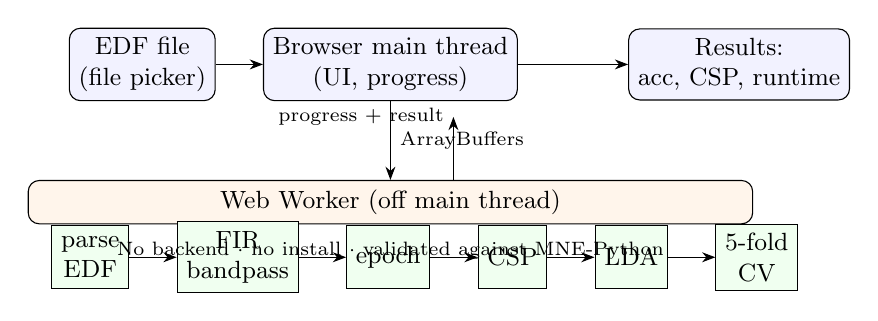
\begin{tikzpicture}[
  font=\small,
  node distance=6mm,
  box/.style={draw, rounded corners, minimum height=8mm, align=center, fill=blue!5},
  stage/.style={draw, minimum height=8mm, align=center, fill=green!6},
  >=Stealth,
]
  \node[box] (file) {EDF file\\(file picker)};
  \node[box, right=of file] (main) {Browser main thread\\(UI, progress)};
  \node[draw, rounded corners, fill=orange!8, below=10mm of main, minimum width=92mm, align=center] (worker) {Web Worker (off main thread)};

  \node[stage, below=7mm of worker.west, anchor=west, xshift=3mm] (parse) {parse\\EDF};
  \node[stage, right=of parse] (filter) {FIR\\bandpass};
  \node[stage, right=of filter] (epoch) {epoch};
  \node[stage, right=of epoch] (csp) {CSP};
  \node[stage, right=of csp] (lda) {LDA};
  \node[stage, right=of lda] (cv) {5-fold\\CV};

  \node[box, right=14mm of main] (res) {Results:\\acc, CSP, runtime};

  \draw[->] (file) -- (main);
  \draw[->] (main) -- (res);
  \draw[->] (main.south) -- node[right, font=\scriptsize]{ArrayBuffers} (worker.north);
  \draw[->] (worker.north) ++(8mm,0) -- ++(0,8mm) node[left, font=\scriptsize]{progress + result};
  \draw[->] (parse) -- (filter); \draw[->] (filter) -- (epoch);
  \draw[->] (epoch) -- (csp); \draw[->] (csp) -- (lda); \draw[->] (lda) -- (cv);
  \node[font=\scriptsize, below=1mm of worker.south, anchor=north] {No backend $\cdot$ no install $\cdot$ validated against MNE-Python};
\end{tikzpicture}
}
\caption{Client-side architecture: the browser parses EEG and runs filter$\rightarrow$epoch%
$\rightarrow$CSP$\rightarrow$LDA$\rightarrow$cross-validation in a Web Worker. No backend, no install.}
\label{fig:arch}
\end{figure}

\subsection{Functionalities}
\textbf{Parsing.} European Data Format (EDF/EDF+) files are decoded in pure JavaScript, including
the annotation track from which motor-imagery events are recovered.
\textbf{Pipeline.} Continuous signals are bandpass filtered with a zero-phase FIR filter
(\FirLo--\FirHi~Hz, \FirTaps{} taps), epoched (\Tmin--\Tmax~s, \Ntimes{} samples per epoch),
projected with CSP (\CspComp{} components, shrinkage regularization \CspReg{}), and classified with
LDA (least-squares solver, shrinkage \LdaShrink{}) under stratified \Folds-fold cross-validation
(seed \Seed{}). These settings are read from a single configuration shared with the reference
oracle, not hard-coded independently.
\textbf{Validation method.} A Python oracle (MNE-Python~\MneVer{}, scikit-learn~\SklearnVer{},
SciPy~\ScipyVer{}, NumPy~\NumpyVer{}, Python~\PyVer{}) runs the identical pipeline and dumps
fixtures (filter coefficients, fold indices, CSP filters, LDA weights, accuracies). The browser
pipeline is compared against these fixtures with explicit tolerances: Pearson correlation on
filtered signals, a sign/order-aligned Frobenius norm on CSP matrices, and a paired $t$-test on
fold accuracies. Filter coefficients and fold splits are reused verbatim so the comparison isolates
implementation fidelity.

% ======================================================================
\section{Illustrative examples}
On the PhysioNet EEG Motor Movement/Imagery Database (imagery runs R04/R08/R12, left- vs.\
right-hand imagery; \Nchannels{} channels at \Fs~Hz; \Nepochs{} epochs per subject), the tool was
run on subjects S001--S010. All \Nsubjects{} subjects validated and \Nskipped{} were skipped. For
\emph{every} subject the browser pipeline reproduced the MNE oracle to machine precision: filter
$r=\FilterR$, CSP Frobenius difference in [\CspFrobMin{}, \CspFrobMax{}], LDA weight difference in
[\LdaDiffMin{}, \LdaDiffMax{}], and identical per-fold and mean cross-validation accuracies
(Fig.~\ref{fig:acc}). Decoding accuracy itself spans \AccMin--\AccMax\%\ across subjects, the
expected between-subject variability of motor-imagery BCI; the tool's claim is numerical
equivalence to the reference, not decoding performance. Figure~\ref{fig:csp} shows the recovered
S001 CSP spatial filters.

\begin{figure}[!t]
\centering
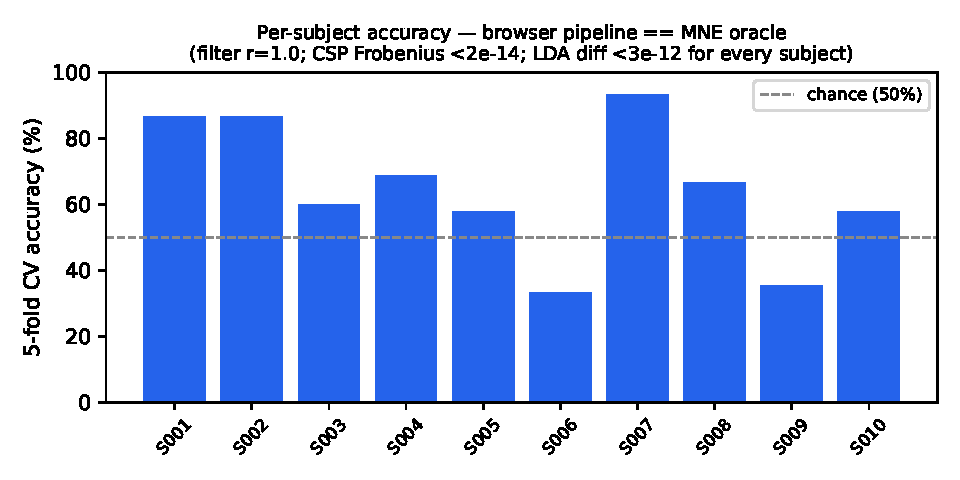
\includegraphics[width=\linewidth]{../shared/figures/accuracy.pdf}
\caption{Per-subject \Folds-fold cross-validation accuracy (S001--S010). For every subject the
browser result equals the MNE oracle to machine precision; accuracy variation reflects
between-subject decodability, not implementation differences.}
\label{fig:acc}
\end{figure}

\begin{figure}[!t]
\centering
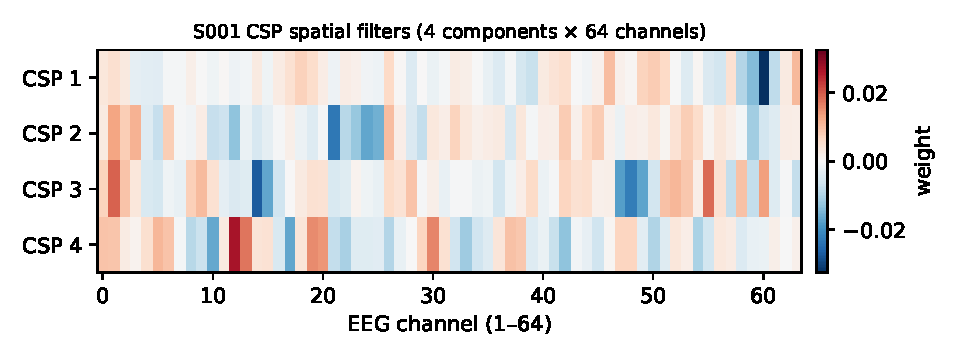
\includegraphics[width=\linewidth]{../shared/figures/csp_s001.pdf}
\caption{CSP spatial filters for subject S001 (\CspComp{} components, \Nchannels{} channels),
read from the validation fixtures.}
\label{fig:csp}
\end{figure}

A real in-browser benchmark (Playwright-driven headless Chromium; \HwCpu{}, \HwCores{}~cores,
\HwRam~GB; \HwBrowser{}; N=\Nreps{} repetitions) gives a full-pipeline runtime of
\WorkerOneX$\pm$\WorkerOneXStd~ms in the Web Worker, with a peak JavaScript heap of \PeakHeap~MB
(Fig.~\ref{fig:perf}). Because CPU throttling via the browser devtools protocol does not reach Web
Workers, a CPU-slowdown proxy was measured by running the identical computation on the throttled
main thread (\ProxyOneX{}/\ProxyFourX{}/\ProxySixX~ms at $1\times$/$4\times$/$6\times$). These
throttled figures are a proxy, \emph{not} a physical low-specification device~\todo{physical
low-spec device run}.

\begin{figure}[!t]
\centering
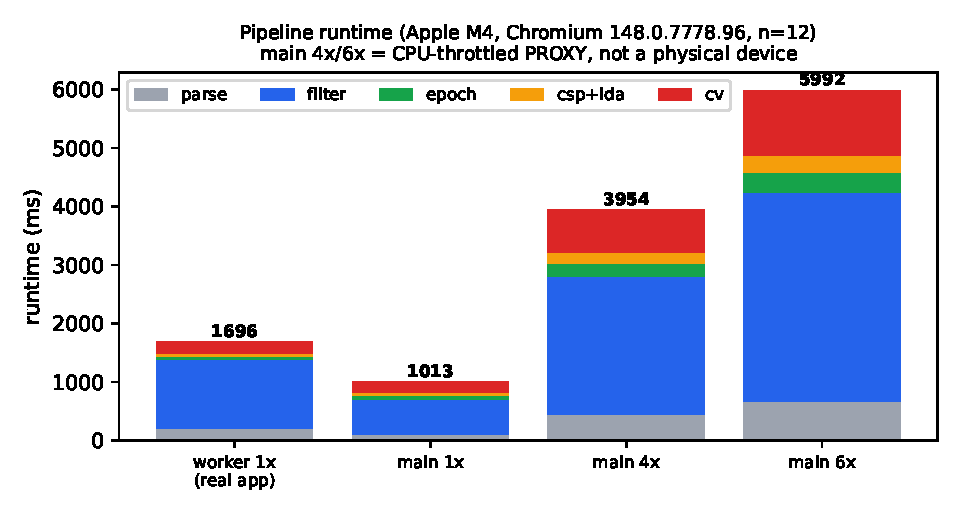
\includegraphics[width=\linewidth]{../shared/figures/performance.pdf}
\caption{Measured runtime (real hardware). Web Worker (real app) at $1\times$ and the identical
computation on the throttled main thread as a CPU-slowdown proxy. Per-stage means stacked; the
$4\times$/$6\times$ bars are a proxy, not a physical device.}
\label{fig:perf}
\end{figure}

% ======================================================================
\section{Impact}
The tool removes installation as a precondition for running standard EEG motor-imagery analysis:
any modern browser suffices, which helps reproducibility (a reader can re-run an analysis from a
link), teaching (no environment setup), and use on restricted or low-resource machines. The
validation methodology---treating an established library as an oracle and checking machine-precision
equivalence per subject---is reusable for any port of a scientific pipeline to a new runtime. The
measured peak heap of \PeakHeap~MB suggests the tool fits within a low-specification RAM budget,
although confirming this on a physical device remains future work (a documented assumption rather
than a tested claim).

% ======================================================================
\section{Conclusions}
We described an install-free, fully client-side EEG motor-imagery analysis tool whose pipeline
reproduces an MNE-Python/scikit-learn reference to machine precision across \Nsubjects{} subjects,
with real in-browser performance measurements. The work packages standard algorithms into a
validated, reproducible, accessible artifact rather than proposing a new method.

% ======================================================================
% SoftwareX mandatory code-metadata table. \todo must be defined in the including document.
\begin{table}[!ht]
\centering
\caption{Code metadata}
\label{tab:codemeta}
\begin{tabular}{|p{0.05\textwidth}|p{0.5\textwidth}|p{0.32\textwidth}|}
\hline
\textbf{Nr} & \textbf{Code metadata description} & \textbf{Value} \\ \hline
C1 & Current code version & \todo{vX.Y.Z (tag a release)} \\ \hline
C2 & Permanent link to code/repository & \todo{GitHub repository URL (GitHub, not GitLab)} \\ \hline
C3 & Permanent link to Reproducible Capsule & \todo{optional (e.g. Code Ocean) -- author decision} \\ \hline
C4 & Legal Code License & \todo{MIT or Apache-2.0 (add LICENSE file)} \\ \hline
C5 & Code versioning system used & git \\ \hline
C6 & Software code languages, tools, services used & TypeScript (strict), Python (oracle), Vite, vitest, ml-matrix, edfdecoder, MNE-Python, scikit-learn \\ \hline
C7 & Compilation requirements, operating environments & Any modern web browser to run; Node.js + npm to build; Python~\PyVer{} venv to regenerate the validation oracle \\ \hline
C8 & Link to developer documentation/manual & \todo{docs URL (e.g. repo README / GitHub Pages)} \\ \hline
C9 & Support email for questions & \todo{author support email} \\ \hline
\end{tabular}
\end{table}


\section*{CRediT author statement}
\textbf{Eugene Cha:} Conceptualization, Methodology, Software, Validation, Investigation, Data
curation, Writing -- original draft, Writing -- review \& editing, Visualization.
\todo{adjust CRediT roles if co-authors are added}

\section*{Data availability}
This study uses the publicly available PhysioNet EEG Motor Movement/Imagery Database
\cite{schalk2004bci2000,goldberger2000physionet}; no new data were generated. Dataset license:
\todo{verify ODC-By / PhysioNet license terms}. Source code: \todo{public GitHub repository URL}.

\section*{Declaration of competing interest}
The author declares no competing interests.

\bibliographystyle{elsarticle-num}
\bibliography{../shared/refs}

\end{document}
